%%% Local Variables:
%%% mode: latex
%%% TeX-master: main
%%% End:

\section*{Circuitos Combinacionais}

\exercise~Explique as principais diferenças entre:

\begin{enumerate}[a)]
\item Multiplexador e demultiplexador;
\item Decodificador e codificador.
\end{enumerate}

\exercise~(multiplexador)~Projete um multiplexador 4\to 1 modulando as
entradas de seleção utilizando um decodificador 2\to 4. Não é
necessário desenhar o circuito do decodificador. Descreva a função
Booleana de saída do mux em função das linhas de entrada e de seleção
provenientes do decodificador.

\exercise~(decodificador)~Projete um decodificador com 2 linhas de
entrada $x$ e $y$, para que somente uma saída esteja no nível {\bf
baixo}, para cada entrada da tabela-verdade.

\exercise~(decodificador)~Projete um decodificador 16\to 4 para
converter a unidade hexadecimal para binário. Construa a
tabela-verdade para este circuito. Não é necessário desenhar o
circuito do decodificador, somente o símbolo.

\pagebreak\exercise~(decodificador)~Para o decodificador~74ALS138 mostrado na
Figura~\ref{74ALS138}, construa a tabela-verdade para as entradas 
de habilitação ({\em ENABLE}) $\overline{e_1}, \overline{e_2}, e_3$ e indique os estados das 
saídas para as seguintes entradas:

\begin{enumerate}[a)]
\item $e_3=\overline{e_2}=1,\quad \overline{e_1}=0,\qquad a_2=a_1=1, a_0=0$;
\item $e_3=1,\quad \overline{e_2}=\overline{e_1}=0,\qquad a_2=0, a_1=a_0=1$.
\end{enumerate}

\begin{figure}[ht]
\begin{center}
\begin{tikzpicture}
  \def\w{2cm}\footnotesize
  \def\h{\w/2}
  \def\r{2.5pt}
  \node[rectangle, minimum height=\h, minimum width=2.5*\w, draw] (DECODER) {decodificador 74ALS138};
  \foreach \X/\x in {2/0,1/.5,0/1}{
    \path[draw] (DECODER.north west)+(\x,0) -- +(\x, \h) node[above] {$x_\X$};
  }
  \foreach \f/\x in {7/0,6/.5,5/1,4/1.5,3/2,2/2.5,1/3,0/3.5}{
    \draw (DECODER.south west)[yshift=-\r,xshift=\x cm] circle (\r) node (INV\f) {};
    \path[draw] (INV\f) -- +(0, -\h) node[below] {$\overline{f_\f}$};
  }
  \node[minimum height=\h,anchor=east,draw,and gate US,rotate=-90] (AND) at (DECODER.north east)[yshift=-\h] {};
  \foreach \p/\e in {south west/1, mid west/2}{
    \draw[]  (AND.\p)[yshift=\r] circle (\r) node (AINV\p) {};
    \path[draw] (AND.\p)+(0,2*\r) -- +(0,\h/2) node[above] {$\overline{e_\e}$};
  }
  \path[draw] (AND.north west) -- +(0,\h/2) node[above] {$e_3$};
\end{tikzpicture}
\end{center}
\label{74ALS138}
\caption{Decodificador 74ALS138.}
\end{figure}

\exercise~(codificador)~O código Gray é um sistema de numeração binário onde dois
valores sucessivos diferem em somente um bit conforme mostrado na
Tabela~\ref{tab:graycode}. Utilizando um decodificador 3\to 8 e um
codificador 8\to 3, projete um circuito que converte o código Gray em
binário. Desenhe somente os símbolos dos circuitos utilizados.

\begin{table}[ht]
  \centering
  \begin{tabular}[ht]{ccc}\hline
    decimal & Gray & binário \\\hline
    0 &  000  &  000\\
    1 &  001  &  001\\
    2 &  011  &  010\\
    3 &  010  &  011\\
    4 &  110  &  100\\
    5 &  111  &  101\\
    6 &  101  &  110\\
    7 &  100  &  111\\\hline
  \end{tabular}
  \caption{Conversão do código Gray para binário.}
  \label{tab:graycode}
\end{table}

\pagebreak\exercise~(demultiplexador)~Descreva com suas próprias
palavras o que o demux da Figura~\ref{fig:printers} é capaz de
realizar. Desenhe o circuito utilizado para o demux utilizando portas
lógicas.

\begin{figure}[ht]
\centering
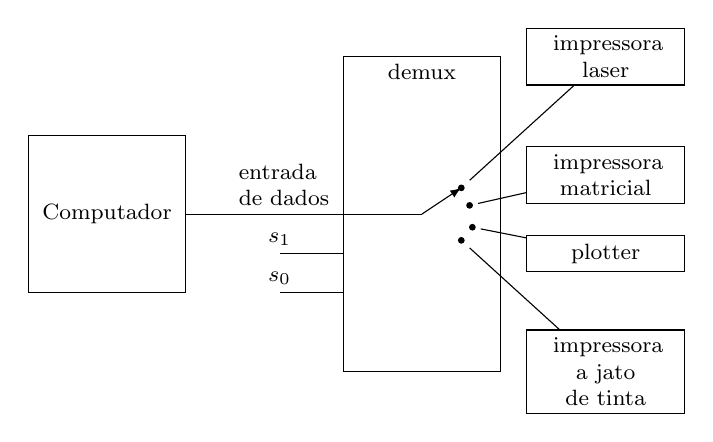
\begin{tikzpicture}
  \tikzset{dev/.style={text centered,minimum width=\len,text width=\len/1.5,draw}}
  \def\len{2cm}\footnotesize
  \node[minimum width=\len,minimum height=\len,draw] (PC) {Computador};
  \node[minimum width=\len,minimum height=2*\len,draw] 
  at (PC)[xshift=2*\len] (DEMUX) {};
  \node[below] at (DEMUX.north) {demux};
  \path[draw] (PC.east)[xshift=\len/1.5] node[text width=\len/1.5,above] {entrada de dados} -- (DEMUX.center) node (basearrow) {};
  \path[->,>=latex,draw] (basearrow.center) -- +(\len/4,\len/6) node (TIP) {};
  \draw[fill] (TIP) circle (1pt) node (laserbase) {};
  \draw[fill] (TIP)[xshift=3pt,yshift=-\len/9] circle (1pt) node (matrixbase) {};
  \draw[fill] (TIP)[xshift=4pt,yshift=-\len/4] circle (1pt) node (plotterbase) {};
  \draw[fill] (TIP)[yshift=-\len/3] circle (1pt) node (jetbase) {};
  %devices
  \node[dev] [right of=DEMUX,xshift=\len/1.5,yshift=\len] (LASER) {impressora laser};
  \node[dev] [right of=DEMUX,xshift=\len/1.5,yshift=\len/4] (MATRIX) {impressora matricial};
  \node[dev] [right of=DEMUX,xshift=\len/1.5,yshift=-\len/4] (PLOTTER) {plotter};
  \node[dev] [right of=DEMUX,xshift=\len/1.5,yshift=-\len] (JET) {impressora a jato de tinta};
  %links
  \path[draw] (laserbase) -- (LASER);
  \path[draw] (matrixbase) -- (MATRIX);
  \path[draw] (plotterbase) -- (PLOTTER);
  \path[draw] (jetbase) -- (JET);
  %selects
  \path[draw] (DEMUX.west)+(0,-\len/4) -- +(-\len/2.5,-\len/4) node[above] {$s_1$};
  \path[draw] (DEMUX.west)+(0,-\len/2) -- +(-\len/2.5,-\len/2) node[above] {$s_0$};
\end{tikzpicture}
\caption{Chaveamento de impressoras.}
\label{fig:printers}
\end{figure}
